\begin{note}
    此小节还未完成。
\end{note}

\subsection{滤波器的表示}

\begin{definition}
    \bd{滤波器}是以特定方式改变信号的频率特性,从而变换信号的处理系统。
    滤波器一般有如下类别,如图 \ref{fig:filter-types} 所示:
    \begin{enumerate}[label=(\arabic*)]
        \item 高通滤波器(HP)
        \item 低通滤波器(LP)
        \item 带通滤波器(BP)
        \item 带阻滤波器(BS)
        \item 全通滤波器(AP)
    \end{enumerate}
    \begin{figure}[H]
        \centering
        \includegraphics[width=0.8\textwidth]{chap4/img/filter_types.png}
        \caption{滤波器类型}
        \label{fig:filter-types}
    \end{figure}

    滤波器也可以被分为\bd{模拟滤波器}和\bd{数字滤波器}。
    \begin{itemize}
        \item \bd{模拟滤波器}是由电阻、电容、电感等部件构成的电路。
            滤波器特性对所用部件的物理标称值非常敏感,而且,
            有些部件的物理特性会随温度变化而改变。
        \item \bd{数字滤波器}是用软件实现的,很少依赖硬件。滤波软件
            只是一系列程序指令。虽然它是在硬件平台上运行,但
            是硬件平台本身并不决定滤波器的性能。数字滤波器的
            性能是由\bd{一组系数}确定的。
    \end{itemize}
    数字滤波器的实现方式一般有以下几种:
    \begin{enumerate}
        \item 用流图计算滤波器的输出。
        \item 用差分方程计算滤波器的输出。
        \item 用卷积过程计算滤波器的输出。
        \item 用 DTFT 直接改变信号频谱。
    \end{enumerate}
\end{definition}

\subsubsection{系统的分类}

\subsubsection{系统的描述方法}

\subsubsection{系统响应的分类}

\subsubsection{FIR 和 IIR 滤波器}

\begin{example}
    \label{exercise:serial-flow-chart}
    写出如图 \ref{fig:serial-flow-chart} 所示级联流图的差分方程。
    \begin{figure}[H]
        \centering
        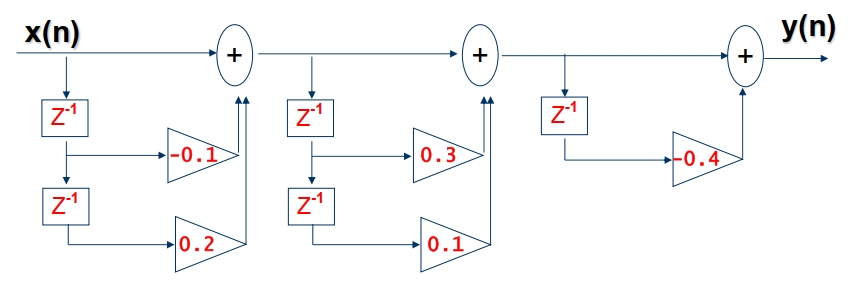
\includegraphics[width=0.8\textwidth]{chap4/img/serial_flow_chart.png}
        \caption{例 \theexample~ 的级联流图}
        \label{fig:serial-flow-chart}
    \end{figure}
\end{example}

\begin{solution}
    不妨设 $x(n) = x_1(n), y(n) = y_3(n)$,
    以及 $y_1(n) = x_2(n), y_2(n) = x_3(n)$,则如图 \ref{fig:serial-flow-chart-annotated} 所示,
    \begin{align*}
        y_1(n) & = x_1(n) - 0.1x_1(n - 1) + 0.2x_1(n - 2), \\
        y_2(n) & = x_2(n) + 0.3x_2(n - 1) + 0.1x_2(n - 2), \\
        y_3(n) & = x_3(n) - 0.4x_3(n - 1).
    \end{align*}
    \begin{figure}[H]
        \centering
        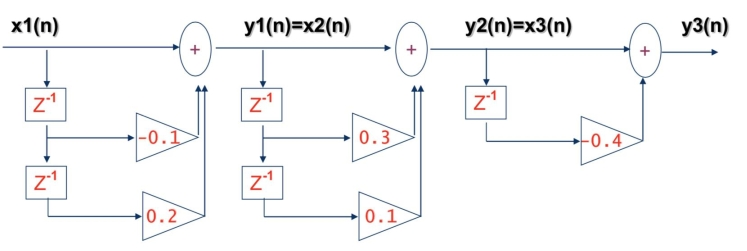
\includegraphics[width=0.8\textwidth]{chap4/img/serial_flow_chart_annotated.png}
        \caption{例 \theexample~ 的级联流图(带标注)}
        \label{fig:serial-flow-chart-annotated}
    \end{figure}
    将 $y_1(n)$ 代入 $y_2(n)$ 的表达式中,将 $y_2(n)$ 代入 $y_3(n)$ 的表达式中,
    可得级联流图的差分方程为
    \begin{align*}
        y_3(n) = x_1(n) - 0.2x_1(n - 1) + 0.19x_1(n - 2) - 0.058x_1(n - 3) - 0.008x_1(n - 5).
    \end{align*}
\end{solution}

% TODO: 4.1 第一个 PPT

\subsubsection{用差分方程表示系统}

\subsubsection{用流图表示系统}

\subsubsection{用脉冲响应表示系统}

\begin{theorem}
    设某滤波器的脉冲响应为 $h(n)$,某输入信号为 $x(n)$。则输入信号可以表示
    为一系列脉冲函数之和:
    \begin{align*}
        x(n) = \sum_{k = -\infty}^{+\infty}x(k)\delta(n - k).
    \end{align*}
    当输入单位脉冲时,即 $x(n) = \delta(n)$,滤波器的输出响应为 $h(n)$,
    则根据 LTI 系统的线性性质和时不变性特性,输入 $x(n)$ 时的输出为
    \begin{align*}
        y(n) = \sum_{k = -\infty}^{+\infty}x(k)h(n - k) = x(n) * h(n).
    \end{align*}
    
    即,\bd{数字滤波器的输出等于输入信号,与脉冲响应的卷积}。
\end{theorem}

\begin{property}[差分方程与卷积运算]
    \label{property:diff-equation-convolution}
    写出 FIR 和 IIR 系统的差分方程如下:
    \begin{align*}
        \sum_{k = 0}^{N}b(k)y(n - k) & = \sum_{k = 0}^{M}a(k)x(n - k) & \text{(IIR)} \\
        y(n) & = \sum_{k = 0}^{M}a(k)x(n - k) & \text{(FIR)}
    \end{align*}
    在 FIR 系统的差分方程中,实际上系数 $a(k)$ 就是系统的脉冲响应 $h(k)$。也就是说,有
    \begin{align*}
        y(n) = a(n) * x(n) \qquad \text{(FIR)}
    \end{align*}

    卷积和差分方程都可以用来计算滤波器的输出。对于 FIR 而言,卷积运算和差分方程都适用;
    对于 IIR 而言,差分方程更加方便。
\end{property}

\begin{remark}
    由以上讨论可知,描述系统的方式有以下几种:
    \begin{itemize}
        \item 系统的差分方程
        \item 流图
        \item 数字系统的脉冲响应 $h(n)$
    \end{itemize}
\end{remark}

\begin{exercise}
    \label{exercise:LTI-stable}
    证明:某 LTI 系统稳定的充要条件是
    \begin{align*}
        \sum_{n = -\infty}^{\infty} \abs{h(n)} = P < \infty.
    \end{align*}
    其中 $h(n)$ 为系统的单位脉冲响应,$P$ 为一个常数。
\end{exercise}

\begin{proof}
    首先证明必要性。不妨设 $\sum_{n= -\infty}^{+\infty}\abs{h(n)} = A$,
    对任意的有界输入 $x(n)$,设 $\forall n, \abs{x(n)} < B$。则
    \begin{align*}
        \abs{y(n)} & = \abs{x(n) * h(n)} = \abs{\sum_{k = -\infty}^{+\infty}h(k)x(n - k)} \\
        & \le \sum_{k = -\infty}^{+\infty} \abs{h(k)} \cdot \abs{x(n - k)} \\
        & < B \sum_{k = -\infty}^{+\infty} \abs{h(k)} = AB
    \end{align*}
    也有界。

    接下来证明充分性。使用反证法,设 $\sum_{n = -\infty}^{\infty} \abs{h(n)}$ 发散时,系统稳定。
    考虑输入
    \begin{align*}
        x(n) = \begin{cases}
                0, & h(-n) = 0, \\
                \sgn{h(-n)}, & h(-n) \neq 0.
            \end{cases}
    \end{align*}
    显然输入是有界的,且 $\forall n, \abs{x(n)} \le 1$。而
    \begin{align*}
        y(0) & = (x * h)(0) = \sum_{k = -\infty}^{+\infty}h(k)x(-k) \\
        & = \sum_{k = -\infty}^{+\infty}h(k) \cdot \sgn{h(k)} \\
        & = \sum_{k = -\infty}^{+\infty}\abs{h(k)}
    \end{align*}
    这个结果发散,说明输出是无界的,这与系统稳定相矛盾。故假设不成立,
    也就是说 $\sum_{n = -\infty}^{\infty} \abs{h(n)}$ 是收敛的。

    命题得证。
\end{proof}

\begin{property}[系统的串、并联组合]
    \label{property:parallel-serial-system}
    系统在串联和并联的情况下,其传递函数的组合规律如下:
    \begin{itemize}
        \item 两个系统的\bd{并联}后新系统的单位冲激响应是并联子系统的单位冲激响应之和,
            传递函数是并联子系统的传递函数之和。如图 \ref{fig:parallel-system} 所示,
            是一个并联系统。
            \begin{align*}
                h(n) = h_1(n) + h_2(n), \quad H(z) = H_1(z) + H_2(z).
            \end{align*}
        \item 两个系统的\bd{串联}后新系统的单位冲激响应是串联子系统的单位冲激响应的卷积,
            传递函数是串联子系统的传递函数的乘积。如图 \ref{fig:serial-system} 所示,
            是一个串联系统。
            \begin{align*}
                h(n) = h_1(n) * h_2(n), \quad H(z) = H_1(z) \cdot H_2(z).
            \end{align*}
    \end{itemize}
    \begin{figure}[H]
        \centering
        \begin{subfigure}{0.45\textwidth}
            \centering
            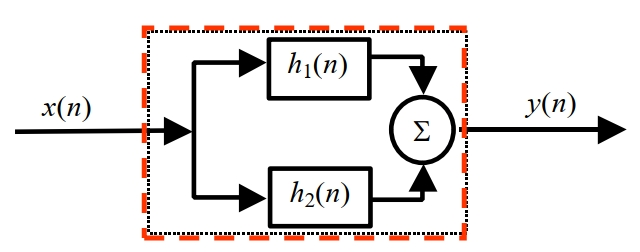
\includegraphics[width=\textwidth]{chap4/img/parallel_system.png}
            \caption{并联系统}
            \label{fig:parallel-system}
        \end{subfigure}
        \begin{subfigure}{0.45\textwidth}
            \centering
            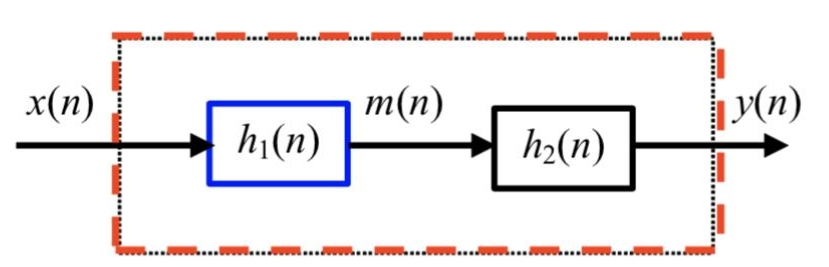
\includegraphics[width=\textwidth]{chap4/img/serial_system.png}
            \caption{串联系统}
            \label{fig:serial-system}
        \end{subfigure}
        \caption{系统的串、并联组合}
    \end{figure}
\end{property}

\subsubsection{系统的频率响应}

\begin{definition}[系统的频率响应]
    \bd{系统的频率响应},简称\bd{频响},反映了系统对激励中各频率分量的幅度和相位的影响。
    通常为复值函数,写成
    \begin{align*}
        H(\omega) = \abs{H(\omega)}\mathe^{\mathi \varphi(\omega)}.
    \end{align*}
    其中,$\abs{H(\omega)}$ 是\bd{幅频响应},$\varphi(\omega)$ 是\bd{相频响应}。
    
    接下来,我们将从 DTFT 的角度来理解频率响应函数和差分方程之间的关系。
    \begin{align*}
        H(\omega) = \sum_{n = -\infty}^{+\infty}h(n)\mathe^{\mathi n \omega}.
    \end{align*}
    由上式可以看出,$H(\omega)$ 是周期函数,分别关于 $\omega = 0$ 和 $\omega = \omega_s/2$ 共轭对称。
\end{definition}

\begin{example}[FIR 系统的频率响应]
    设有 FIR 系统,其差分方程为
    \begin{align*}
        y(n) = \sum_{k = -\infty}^{+\infty}x(k)h(n - k),
    \end{align*}
    即 $y(n) = x(n) * h(n)$。对等式左右求 DTFT,得
    \begin{align*}
        Y(\omega) = X(\omega) H(\omega).
    \end{align*}
    因此,滤波器的\bd{频率响应}为
    \begin{align*}
        H(\omega) = Y(\omega) / X(\omega) = \DTFT{h(n)}.
    \end{align*}
\end{example}

\begin{theorem}[频率响应与差分方程]
    \label{thm:freq-response-diff-equation}
    设有差分方程
    \begin{align*}
        \sum_{k = 0}^{N}b(k)y(n - k) = \sum_{k = 0}^{M}a(k)x(n - k),
    \end{align*}
    其中 $x(n), y(n)$ 的 DTFT 分别为 $X(\omega), Y(\omega)$,则系统的频率响应为
    \begin{align*}
        H(\omega) = \frac{Y(\omega)}{X(\omega)} = \frac{\sum_{k = 0}^{M}a(k)\mathe^{-\mathi k \omega}}{\sum_{k = 0}^{N}b(k)\mathe^{-\mathi k \omega}}.
    \end{align*}
\end{theorem}

\begin{proof}
    考虑差分方程
    \begin{align*}
        \sum_{k = 0}^{N}b(k)y(n - k) = \sum_{k = 0}^{M}a(k)x(n - k),
    \end{align*}
    即 $b(n) * y(n) = a(n) * x(n)$。对等式左右求 DTFT,得
    \begin{align*}
        Y(\omega) \sum_{k = 0}^{N}b(k)\mathe^{-\mathi k\omega} = X(\omega)\sum_{k = 0}^{M}a(k)\mathe^{-\mathi k\omega}.
    \end{align*}
    此即
    \begin{align*}
        H(\omega) = \frac{Y(\omega)}{X(\omega)} = \frac{\sum_{k = 0}^{M}a(k)\mathe^{-\mathi k \omega}}{\sum_{k = 0}^{N}b(k)\mathe^{-\mathi k \omega}}.
    \end{align*}
    命题得证。
\end{proof}

\begin{remark}
    对于定理 \ref{thm:freq-response-diff-equation},我们可以进一步讨论。
    对于差分方程
    \begin{align*}
        \sum_{k = 0}^{N}b(k)y(n - k) = \sum_{k = 0}^{M}a(k)x(n - k),
    \end{align*}
    \begin{itemize}
        \item 输出信号可以由输入信号的当前(及过去)与输出信号的过去的线性组合表示。
        \item 输出信号与其延迟信号的叠加,等于输入信号与其延迟信号的叠加。
    \end{itemize}
    它们的 DTFT 相等,说明\bd{原信号在时域叠加,结果信号的频谱也是原信号频谱的叠加}。
\end{remark}

\begin{exercise}
    已知某因果系统的流图如 \ref{fig:chap4-part1-quiz2} 所示,且满足 $0 < a < 1$.
    求系统的差分方程、系统的频率响应、以及系统的幅频响应图,
    并说明系统相当于何种滤波器(高通、低通、带通、带阻、全通)。
    \begin{figure}[H]
        \centering
        \tikzstyle{block} = [draw, rectangle, minimum height=1cm, minimum width=1cm]
        \tikzstyle{circ} = [draw, fill, circle, inner sep=1.5pt]
        \tikzstyle{no-circ} = [draw, circle, inner sep=0pt]
        \tikzstyle{sum} = [draw, circle]
        \tikzstyle{line} = [draw, -latex]
        \tikzstyle{no-arrow-line} = [draw, -]
        \tikzstyle{gainx} = [draw, isosceles triangle, isosceles triangle apex angle=60]
        \tikzstyle{gainy} = [draw, isosceles triangle, isosceles triangle apex angle=60, shape border rotate=180]
        \begin{tikzpicture}
            \node [name=input] (input) {$x(n)$};
    
    
            \node [sum, right of=input, xshift=4cm] (sum) {$+$};
            \node [circ, right of=sum, xshift=4cm] (circy) {};
            \path [no-arrow-line] (sum) -- (circy);
            \node [name=output, right of=circy, xshift=1cm] (output) {$y(n)$};
            \path [line] (circy) -- (output);
    
    
            \node [block, below of=circy, yshift=-1cm] (zy1) {$Z^{-1}$};
            \path [line] (circy) -- (zy1);
    
            \path [line] (input) -- (sum);
            \node [gainy, below of=zy1, xshift=-2cm, yshift=-0.5cm] (zgy1) {$a$};
            \path [line] (zy1) |- (zgy1);
            \path [line] (zgy1.west) -- (sum);
        \end{tikzpicture}
        \caption{习题 \theexercise~ 的信号流图}
        \label{fig:chap4-part1-quiz2}
    \end{figure}
\end{exercise}

\begin{solution}
    由图可知系统的差分方程为
    \begin{align*}
        y(n) = ay(n - 1) + x(n).
    \end{align*}
    因此,系统的频率响应为
    \begin{align*}
        H(\omega) = \frac{\mathe^{\mathi \omega}}{\mathe^{\mathi \omega} - a}
            = \frac{1}{(1 - a\cos\omega) + \mathi a\sin\omega}
    \end{align*}
    所以其幅频响应函数为
    \begin{align*}
        \abs{H(\omega)} & = \frac{1}{\sqrt{(1 - a\cos\omega)^2 + a^2\sin^2\omega}} \\
        & = \frac{1}{\sqrt{1 + a^2 - 2a\cos\omega}}
    \end{align*}
    如图 \ref{fig:chap4-part1-quiz2-plot} 所示,其幅频响应函数为一个低通滤波器。
    \begin{figure}[H]
        \centering
        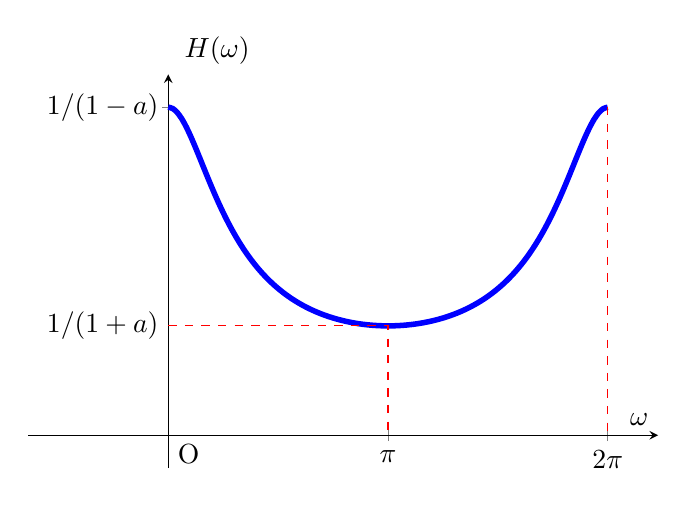
\begin{tikzpicture}
            \begin{axis}[
                axis lines = middle,
                xlabel = {$\omega$},
                ylabel = {$\abs{H(\omega)}$},
                ylabel style={at={(rel axis cs:0.3, 1)}, anchor=south},
                xmin = -2, xmax = 7,
                ymin = -0.2, ymax = 2.2,
                xtick = {0, 3.14, 6.28},
                xticklabels = {$0$, $\pi$, $2\pi$},
                ytick = {0, 2},
                yticklabels = {$ $, $ $},
                scale only axis,
                width = 8cm,
                height = 5cm,
            ]
            \addplot[domain=0:6.28, samples=100, smooth, line width=2pt, blue] {1 / sqrt(1.25 - cos(deg(x)))};
            \addplot[dashed, red] coordinates {(0, 0.667) (3.14, 0.667) (3.14, 0)};
            \addplot[dashed, red] coordinates {(6.28, 2) (6.28, 0)};
            \node at (axis cs:0, 0) [anchor=north west] {O};
            \node at (axis cs:0, 0.667) [anchor=east] {$1/(1 + a)$};
            \node at (axis cs:0, 2) [anchor=east] {$1/(1 - a)$};
            \end{axis}
        \end{tikzpicture}
        \caption{习题 \theexercise~ 的幅频响应函数}
        \label{fig:chap4-part1-quiz2-plot}
    \end{figure}
\end{solution}

\subsubsection{由差分方程求脉冲响应函数}

在性质 \ref{property:diff-equation-convolution} 中我们已经知道,
对于 FIR 系统,$h(n) = a(n)$。那么对于 IIR 系统,
\begin{align*}
    \sum_{k = 0}^{N}b(k)y(n - k) = \sum_{k = 0}^{M}a(k)x(n - k).
\end{align*}
我们应该如何求解 $h(n)$ 呢?可以考虑使用更强大的工具——Z 变换。
